\documentclass[12pt,oneside]{report}
%%%%%%%%%%%%%%%%%%%%%%%%%%%%%%%%%%%%%%%%%%%%%%%%%%%%%%%%%%%%%%%%%%%%%%%%%%%%%%%
\input{preambule_2024}
%%%%%%%%%%%%%%%%%%%%%%%%%%%%%%%%%%%%%%%%%%%%%%%%%%%%%%%%%%%%%%%%%%%%%%%%%%%%%%%
\portrait
%\paysage
%\usepackage{cclicenses}
%%%%%%%%%%%%%%%%%%%%%%%%%%%%%%%%%%%%%%%%%%%%%%%%%%%%%%%%%%%%%%%%%%%%%%%%%%%%%%%
%%%%%%%%À modifier !!!!!!!!!!!!!!!!
\newcommand{\classe}{\LaTeX{}}
\newcommand{\titredoc}{\fontfamily{pzc}
\bfseries\fontsize{30}{20}\selectfont{Examples with pgfplots}%\\[0.2em]
%\today
}
\newcommand{\auteurs}{D.T.}

%%%%%%%%%%%%%%%%%%%%%%%%%%%%%%%%%%%%%%%%%%%%%%%%%%%%%%%%%%%%%%%%%%%%%%%%%%%%%%%
\fancyhf{}
\rhead{ \textcolor{orange!90}{\bsc{\large \classe}}}
\lhead{}
\rfoot{\textcolor{blue}{Licence : \ccbyncsaeu}}

\lfoot{ \textcolor{blue}{\auteurs}}
\cfoot{\thepage / \pageref{LastPage}}
\renewcommand \headrulewidth{0pt}
\renewcommand {\footrule}{{\color{orange!70}\rule{\textwidth}{0.9pt}}}
\pagestyle{fancy}
%\tikzset{domaine/.style 2 args={domain=#1:#2}}

%%%%%%%%%%%%%%%%%%%%%%%%%%%%%%%%%%%%%%%%%%%%%%%%%%%%%%%%%%%%
\usepackage[linesnumbered,french]{algorithm2e}
%%%%%%%%%%%%%%%%%%%%%%%%%%%%%%%%%%%%%%%%%%%%%%%%%%%%%%%%%%%%
\newcommand{\cadrevide}[1]{
\begin{Cadre}
\begin{minipage}{\linewidth}
\vspace{#1}
\end{minipage}
\end{Cadre}}
%%%%%%%%%%%%%%%%%%%%%%%%%%%%%%%%%%%%%%%%%%%%%%%%%%%%%%%%%%%%
\begin{document}
\selectlanguage{english}

\begin{Cadre}
\begin{minipage}{0.98\linewidth}
\begin{center}
\textcolor{blue}{
\titredoc
}
\end{center}
\end{minipage}
\end{Cadre}

%%%%%%%%%%%%%%%%%%%%%%%%%%%%%%%%%%%%%%%%%%%%%%%%%%%%%%%%%%%%
\begin{spacing}{1.2}
%%%%%%%%%%%%%%%%%%%%%%%%%%%%%%%%%%%%%%%%%%%%%%%%%%%%%%%%%%%%

\section*{Example \#1}\label{example1}


\begin{center}%(-6,-4)--->(3,5)
\begin{tikzpicture}[>=stealth]
\begin{axis}[xmin=-6,xmax=3,
ymin=-4,ymax=5,
grid,
xtick distance=1,ytick distance=1,
axis lines = middle,
axis line style = {->, line width = 1.5pt, color=blue},
scale=2]
\addplot gnuplot [id=c1, color=red, domain=-6:3, line width=2pt, no marks, samples=500]{-2*exp(0.5*x)+1} node[pos=0.7, above right]{$\mathcal{C}_1$};
\addplot gnuplot [id=c2, color=OliveGreen, domain=-6:3, line width=2pt, mark=none, samples=500]{-exp(0.5*x)+1} node[pos=0.8, above right]{$\mathcal{C}_2$};
\addplot gnuplot [id=c3, color=blue, domain=-6:3, line width=2pt, mark=none, samples=500]{exp(0.5*x)+1} node[pos=0.8, below right]{$\mathcal{C}_3$};
\addplot gnuplot [id=c4, color=violet, domain=-6:1, line width=2pt, mark=none, samples=500]{3*exp(0.5*x)+1} node[pos=0.85, below right]{$\mathcal{C}_4$};
\end{axis}
\end{tikzpicture}
\end{center}


\section*{Example \#2}\label{example2}

\begin{center}
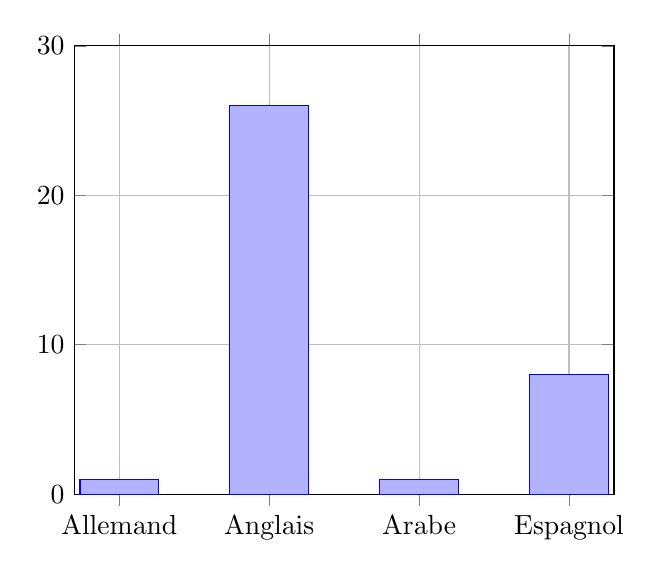
\begin{tikzpicture}
\begin{axis}[ybar,xtick={1,2,3,4},xticklabels={Allemand,Anglais,Arabe,Espagnol},
ymin=0,ymax=30,grid=major,bar width=1cm]
\addplot coordinates{(1,1)(2,26)(3,1)(4,8)};
\end{axis}
\end{tikzpicture}
\end{center}

\section*{Example \#3}\label{example3}

\begin{center}
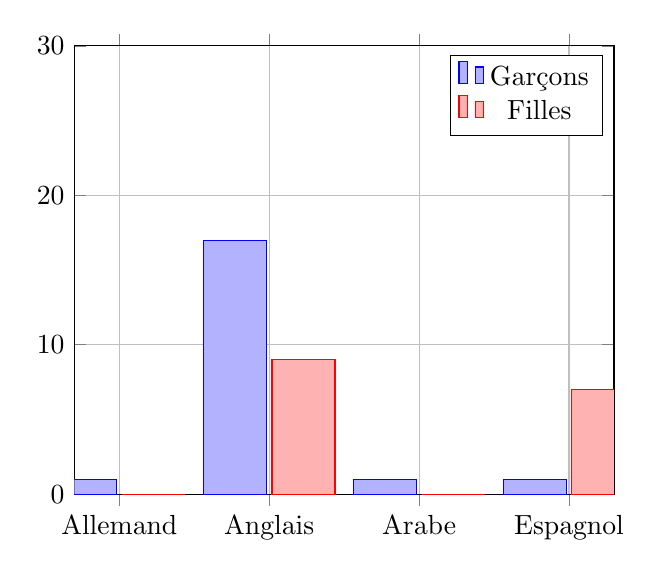
\begin{tikzpicture}
\begin{axis}[ybar,grid= major ,
xtick={1,2,3,4},xticklabels={Allemand,Anglais,Arabe,Espagnol},
ymin=0,ymax=30,
%legend style={at={(0.5,1.03)},anchor=south},
legend entries={Garçons,Filles},bar width=0.8cm]
\addplot coordinates{(1,1)(2,17)(3,1)(4,1)};
\addplot coordinates{(1,0)(2,9)(3,0)(4,7)};
\end{axis}
\end{tikzpicture}
\end{center}

\section*{Example \#4}\label{example4}

\begin{center}
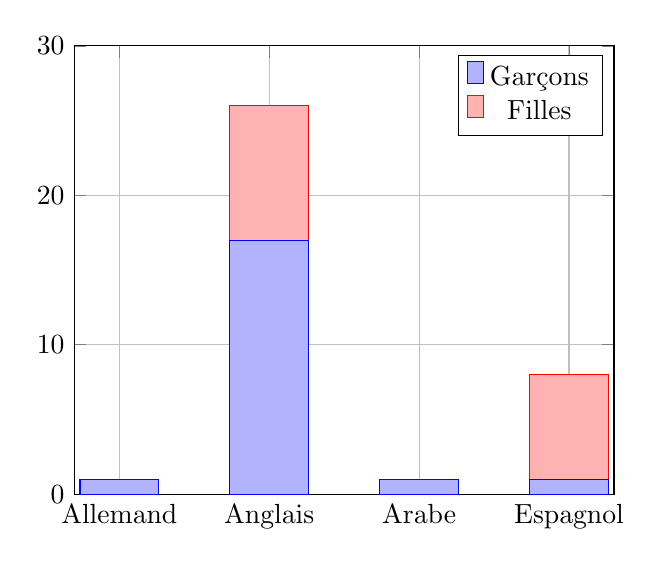
\begin{tikzpicture}
\begin{axis}[ybar stacked,grid= major ,
xtick={1,2,3,4},xticklabels={Allemand,Anglais,Arabe,Espagnol},
ymin=0,ymax=30,ystep=2,
%legend style={at={(0.5,1.03)},anchor=south},
legend entries={Garçons,Filles},bar width=1cm]
\addplot coordinates{(1,1)(2,17)(3,1)(4,1)};
\addplot coordinates{(1,0)(2,9)(3,0)(4,7)};
\end{axis}
\end{tikzpicture}
\end{center}


\section*{Example \#5}\label{example5}


\begin{center}
\begin{center}
\begin{tikzpicture}
\begin{axis}[
xlabel={Taille (en cm)},
ylabel={Masse (en kg)},]
\addplot+[only marks] coordinates {
(48,3)(45,3.2)(50,3.8)(53,4.5)(49,2.6)
};
\end{axis}
\end{tikzpicture}
\end{center}
\end{center}

%%%%%%%%%%%%%%%%%%%%%%%%%%%%%%%%%%%%%%%%%%%%%%%%%%%%%%%%%%%
\end{spacing}
%%%%%%%%%%%%%%%%%%%%%%%%%%%%%%%%%%%%%%%%%%%%%%%%%%%%%%%%%%%%
%%%%%%%%%%%%%%%%%%%%%
%% FIN DU DOCUMENT %%
%%%%%%%%%%%%%%%%%%%%%
\end{document}